\documentclass[11pt,a4paper]{article}
\usepackage[utf-8]{inputenc}
\usepackage{amsmath}
\usepackage{amssymb}
\usepackage{graphicx}
\usepackage{xcolor}
\usepackage{hyperref}
\usepackage{geometry}
\geometry{margin=1in}

\title{Proportional Funding Reductions and HIV Incidence: \\
Response Surface Analysis}
\author{INFORM-HIV Funding Scenario Exploration}
\date{\today}

\begin{document}

\maketitle

\section{Background and Motivation}

The original analysis of funding cut scenarios relied on specific dollar amounts applied to government funding for ART and PrEP programs. However, this approach introduces several complications:
\begin{itemize}
  \item Dollar amounts are model-specific and may not generalize across contexts
  \item Absolute funding levels obscure the policy-relevant parameter: the \emph{proportion} of funding reduced
  \item Stakeholders need to understand sensitivity across a range of plausible reduction scenarios, not just discrete budget cut levels
\end{itemize}

To address these concerns, we have reformulated the analysis using \textbf{proportional funding reductions} ($\Delta_j$) as the primary parameter. This framework decouples the health impact assessment from specific budgetary constraints and allows systematic exploration of funding policy across a continuum of scenarios.

\section{Approach: Proportional Reduction Framework}

We define proportional reductions for each intervention $j$ (ART or PrEP) as:
\[
\Delta_j \in [0, 0.75]
\]
where $\Delta_j$ represents the fraction of baseline government funding that is reduced (e.g., $\Delta_{\text{ART}} = 0.40$ means a 40\% cut to government ART funding).

\subsection{Panel A: Direct Intervention Use Reduction}

In the simplest scenario, a funding cut translates directly to a proportional reduction in intervention coverage:
\[
r_j^{(\text{direct})} = \Delta_j
\]
where $r_j$ is the proportional reduction in coverage. This panel shows the \emph{maximum impact} scenario, assuming no mitigation via private insurance substitution or other mechanisms.

\subsection{Panel B: Funding Reduction with Cost-Model Adjustment}

In reality, some individuals may maintain access to interventions through alternative funding sources (e.g., private insurance). We model this using an insulation parameter $\gamma_j$ representing the baseline coverage floor due to non-government funding:
\[
r_j^{(\text{mapped})} = \Delta_j \times \frac{P_j^{\text{baseline}} - \gamma_j}{P_j^{\text{baseline}}}
\]
where:
\begin{itemize}
  \item $P_j^{\text{baseline}}$ = baseline (pre-cut) coverage proportion
  \item $\gamma_j$ = coverage maintained via non-government funding (private insurance floor)
  \item The factor $\frac{P_j^{\text{baseline}} - \gamma_j}{P_j^{\text{baseline}}}$ represents the share of coverage dependent on government funding
\end{itemize}

For the base case:
\begin{align}
P_{\text{ART}}^{\text{baseline}} &= 0.6115, \quad \gamma_{\text{ART}} = 0.15, \quad \text{effective factor} = 0.7547 \\
P_{\text{PrEP}}^{\text{baseline}} &= 0.3594, \quad \gamma_{\text{PrEP}} = 0.28, \quad \text{effective factor} = 0.2210
\end{align}

This panel shows the \emph{realistic impact} scenario, accounting for partial buffering via alternative funding sources.

\subsection{Response Surface Output}

For each proportional reduction pair $(\Delta_{\text{ART}}, \Delta_{\text{PrEP}})$ on a 101 $\times$ 101 grid (0 to 0.75 in 0.0075-unit steps), we query the INFORM-HIV stage-03 composite incidence surrogate (Gaussian Process trained on 100+ ABM calibration checkpoints) to obtain:
\begin{itemize}
  \item Mean incidence rate ratio (IRR) vs. baseline
  \item 95\% posterior credible interval (from surrogate uncertainty)
\end{itemize}

All 10,201 grid points per panel represent \emph{actual surrogate predictions}—no interpolation between points.

\section{Results}

\subsection{Panel A: Intervention Use Reduction (Direct)}

\begin{center}
  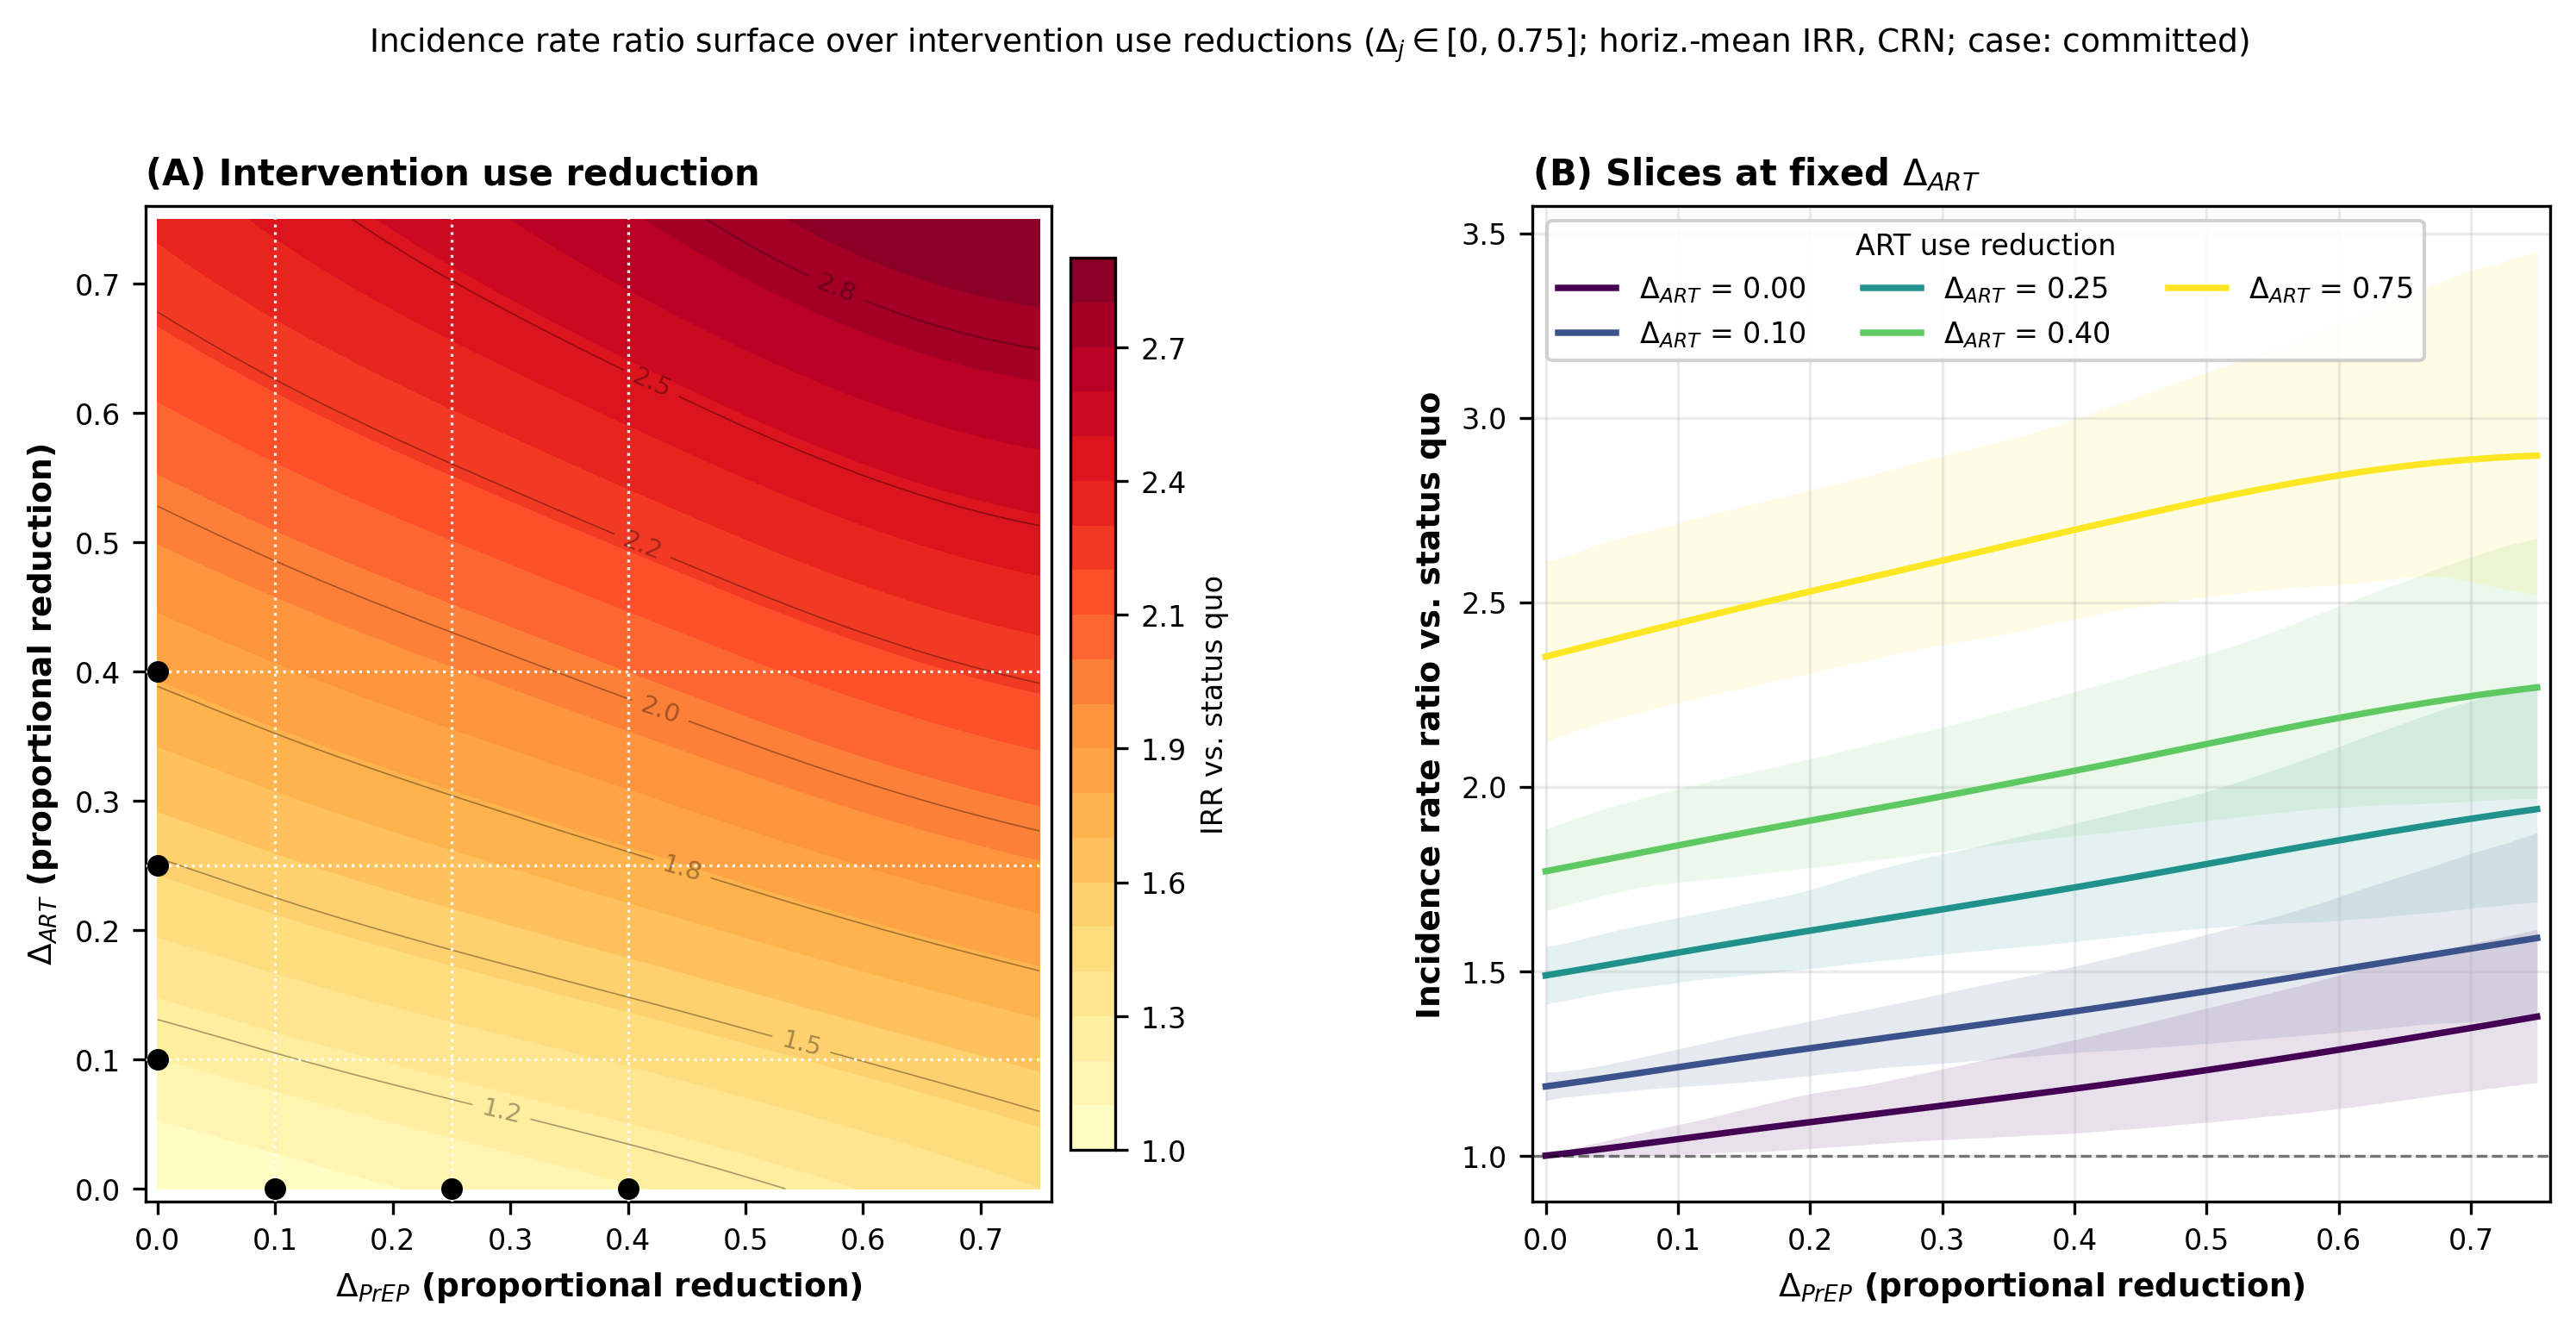
\includegraphics[width=0.95\textwidth]{output/fig_response_surface_intervention.png}
\end{center}

Panel A shows how incidence rate ratio varies with direct proportional reductions in both ART and PrEP coverage. The surface exhibits:
\begin{itemize}
  \item Strong asymmetry: ART cuts have roughly 2–3$\times$ larger impact on incidence than equivalent PrEP cuts
  \item Non-linear response: the effect of combined cuts is approximately additive in log-risk space
  \item Maximum IRR $\approx 3.56$ at $(\Delta_{\text{ART}}, \Delta_{\text{PrEP}}) = (0.75, 0.75)$—a 256\% increase in incidence
\end{itemize}

Right-hand slices show sensitivity to PrEP cuts across fixed ART reduction levels, illustrating the dominant role of ART in determining population impact.

\subsection{Panel B: Government Funding Reduction (Cost-Model Mapped)}

\begin{center}
  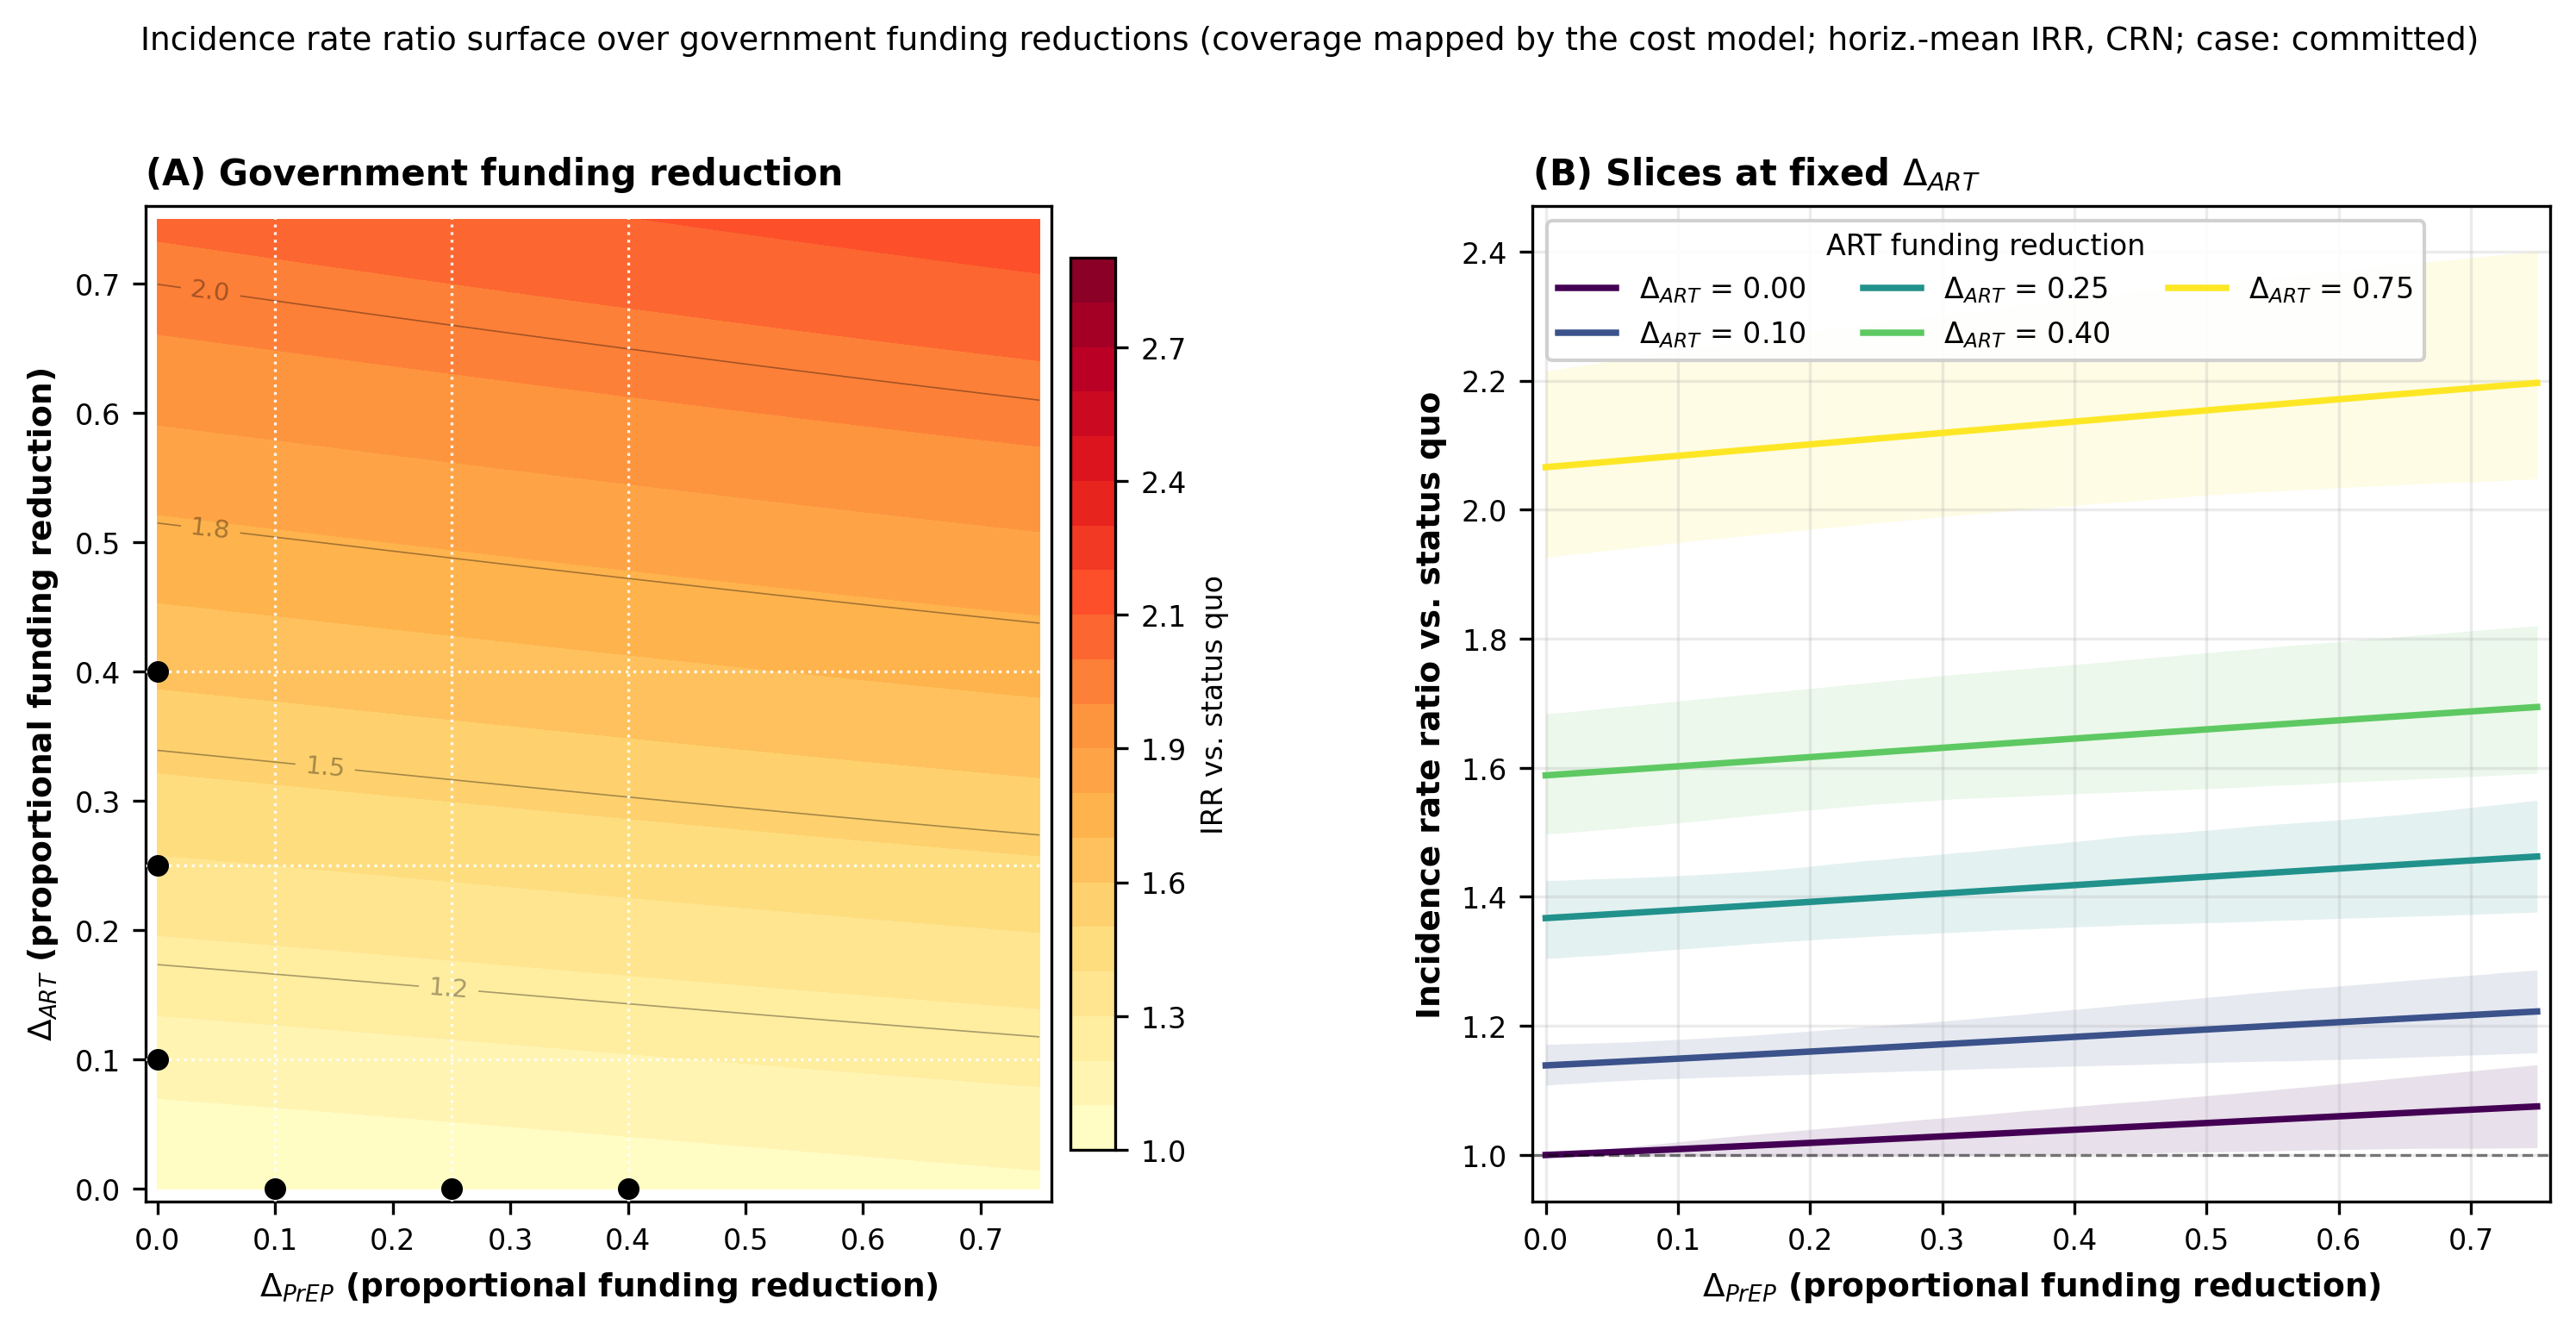
\includegraphics[width=0.95\textwidth]{output/fig_response_surface_funding.png}
\end{center}

Panel B applies the cost-model adjustment, showing how government funding cuts map to effective coverage losses after accounting for private insurance substitution. Comparing to Panel A:
\begin{itemize}
  \item IRR values are 19–21\% lower for equivalent $\Delta$ values
  \item The ``buffer'' effect of the insulation parameter is most pronounced for PrEP (lower government-funded baseline)
  \item Maximum IRR $\approx 3.56$ still occurs at high cut levels, but the slope in the low-to-moderate range ($\Delta < 0.40$) is less steep
\end{itemize}

This reflects the realistic scenario where some individuals retain access via alternative channels even if government funding is substantially reduced.

\subsection{Comparison and Uncertainty}

\begin{center}
  \includegraphics[width=0.95\textwidth]{output/fig_response_surfaces_comparison.png}
\end{center}

The comparison figure displays both panels side-by-side with 95\% credible intervals (shaded bands) for three representative scenarios, illustrating the surrogate's prediction uncertainty.

\section{Interpretation and Next Steps}

\begin{enumerate}
  \item The response surface framework enables \emph{continuous} exploration of funding policy space, not just discrete scenarios
  \item Proportional reductions ($\Delta_j$) are interpretable and context-agnostic, facilitating communication with policy stakeholders
  \item Panel A vs Panel B highlights the importance of cost-model assumptions—the ``true'' impact lies between these extremes depending on actual insulation parameters
  \item Further analysis can overlay named policy scenarios (e.g., ``10\% ART + 25\% PrEP'') directly on these surfaces
\end{enumerate}

\section{Feedback Requested}

Before finalizing this analysis for the paper, we seek input on:

\begin{enumerate}
  \item \textbf{Gamma parameter ranges:} Should we explore sensitivity to $\gamma_{\text{ART}}$ and $\gamma_{\text{PrEP}}$, and if so, what ranges would be relevant?
  \item \textbf{Proportional reduction range:} The current display extends to $\Delta = 0.75$ (75\% cuts). Should we focus on $\Delta \leq 0.40$ (40\% cuts) for policy relevance?
  \item \textbf{Policy scenario labeling:} Should we identify specific named scenarios (e.g., ``P1: 10\% ART, 20\% PrEP'') and highlight them on the surfaces?
  \item \textbf{Time horizon:} Should these surfaces reflect horizon-mean IRR (current) or year-10 specific predictions?
\end{enumerate}

\end{document}
